\documentclass[11pt,a4paper]{article}

\usepackage[margin=2.2cm]{geometry}
\usepackage{amsmath,amssymb,amsthm,mathtools}
\usepackage{booktabs}
\usepackage[dvipsnames]{xcolor}
\usepackage{hyperref}
\usepackage{listings}
\usepackage{tikz}

\hypersetup{
  colorlinks=true,
  linkcolor=blue!60!black,
  urlcolor=blue!60!black
}

\lstdefinestyle{code}{
  language=Python,
  basicstyle=\ttfamily\small,
  keywordstyle=\color{blue!70!black},
  commentstyle=\color{ForestGreen!70!black},
  stringstyle=\color{BrickRed},
  showstringspaces=false,
  breaklines=true,
  frame=single,
  rulecolor=\color{black!20},
  backgroundcolor=\color{black!2}
}

\theoremstyle{definition}
\newtheorem*{problem}{Problem}
\newtheorem*{intuition}{Intuition}
\newtheorem*{definitionblock}{Definition}
\newtheorem*{solution}{Solution}

\theoremstyle{plain}
\newtheorem*{theoremblock}{Theorem}

\title{What Infinite Series Are and How They Appear in Everyday Life}
\author{}
\date{\today}

\begin{document}

\maketitle
\tableofcontents
\newpage

\section{What This Note Is Trying to Solve}

Many beginners hear the phrase \emph{infinite series} and immediately think:
\begin{quote}
How can adding infinitely many numbers ever make sense?
\end{quote}

That is the right first question.

An infinite series is not a mysterious calculator that performs infinitely many additions in one instant.
It is a way to study the behavior of longer and longer \emph{partial sums}.
We keep adding one more term, then one more term, then one more term, and we ask:
\begin{quote}
Do these running totals settle down near one fixed number, or do they keep drifting away?
\end{quote}

If the running totals approach one number, we say the series \emph{converges}.
If not, we say it \emph{diverges}.

This note is written for a first-time learner.
The goal is not to cover every theorem.
The goal is to build a reliable beginner picture:
\begin{enumerate}
  \item what an infinite series is,
  \item why infinitely many terms can still have a finite sum,
  \item when such a sum makes sense,
  \item and where this idea appears in ordinary life and technology.
\end{enumerate}

\section{The Teaching Principle}

Every part of this note follows the same four layers.

\begin{enumerate}
  \item \textbf{Background question.}
  What real confusion are we trying to remove?
  \item \textbf{Naive intuition.}
  What is the plain-language picture before symbols appear?
  \item \textbf{Mathematical expression.}
  What do the symbols mean, term by term?
  \item \textbf{Computation correspondence.}
  How would a calculator or computer actually work with the idea?
\end{enumerate}

This order matters.
If the intuition is missing, the notation feels arbitrary.
If the notation is missing, the intuition stays too vague.
If the computation viewpoint is missing, the topic feels detached from real use.

\section{The Five Questions a Beginner Should Ask First}

\begin{enumerate}
  \item What is the difference between a sequence and a series?
  \item How can infinitely many pieces add up to a finite amount?
  \item When does an infinite series converge, and when does it fail to converge?
  \item Where do infinite series appear in everyday life?
  \item If no machine can add infinitely many terms, why are infinite series still useful?
\end{enumerate}

\section{Question-and-Answer Walkthrough}

\subsection{Question 1: What is the difference between a sequence and a series?}

\begin{problem}
The words \emph{sequence} and \emph{series} sound similar, but they are not the same thing.
\end{problem}

\begin{intuition}
A sequence is just a list of numbers.
A series is what you get when you start adding the numbers from that list.
\end{intuition}

For example, the list
\[
\frac{1}{2},\ \frac{1}{4},\ \frac{1}{8},\ \frac{1}{16},\ \dots
\]
is a \emph{sequence}.

If we add the terms, we get
\[
\frac{1}{2}+\frac{1}{4}+\frac{1}{8}+\frac{1}{16}+\dots,
\]
and that is a \emph{series}.

\begin{definitionblock}
If the terms are \(a_1,a_2,a_3,\dots\), then the infinite series is written as
\[
\sum_{n=1}^{\infty} a_n.
\]
Its \(N\)-th partial sum is
\[
S_N = a_1+a_2+\cdots+a_N.
\]
\end{definitionblock}

The key object is really the sequence of partial sums:
\[
S_1,\ S_2,\ S_3,\ \dots
\]
because convergence means that these running totals approach a fixed number.

\subsection{Question 2: How can infinitely many pieces add up to a finite amount?}

\begin{problem}
It feels natural to think that ``more and more additions'' must force the total to become infinite.
\end{problem}

\begin{intuition}
That would be true if the later pieces stayed large.
But if each new piece becomes small very quickly, then the remaining gap can shrink toward zero.
\end{intuition}

The classic example is
\[
\frac{1}{2}+\frac{1}{4}+\frac{1}{8}+\frac{1}{16}+\dots
\]
Its partial sums are
\[
S_1=\frac{1}{2},\qquad
S_2=\frac{3}{4},\qquad
S_3=\frac{7}{8},\qquad
S_4=\frac{15}{16},\dots
\]
Each partial sum gets closer to \(1\), and the missing part keeps getting cut in half.

\begin{center}
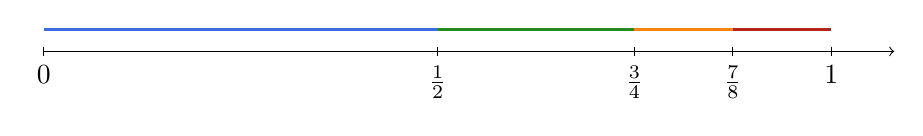
\begin{tikzpicture}[x=10cm,y=1cm]
  \draw[->] (0,0) -- (1.08,0);
  \draw[very thick, RoyalBlue] (0,0.28) -- (0.5,0.28);
  \draw[very thick, ForestGreen] (0.5,0.28) -- (0.75,0.28);
  \draw[very thick, BurntOrange] (0.75,0.28) -- (0.875,0.28);
  \draw[very thick, BrickRed] (0.875,0.28) -- (1,0.28);
  \foreach \x/\lab in {0/{0},0.5/{\frac{1}{2}},0.75/{\frac{3}{4}},0.875/{\frac{7}{8}},1/{1}} {
    \draw (\x,0.06) -- (\x,-0.06);
    \node[below] at (\x,-0.06) {$\lab$};
  }
\end{tikzpicture}
\end{center}

This is the first big idea of infinite series:
\begin{quote}
An infinite series can have a finite sum because the \emph{limit of the partial sums} can be finite.
\end{quote}

A familiar everyday version is the repeating decimal
\[
0.999\ldots = \frac{9}{10}+\frac{9}{100}+\frac{9}{1000}+\dots,
\]
which also converges to a finite number, namely \(1\).

\subsection{Question 3: When does a series converge, and when does it fail to converge?}

\begin{problem}
Not every series behaves nicely.
Some settle down; some do not.
\end{problem}

\begin{definitionblock}
We say
\[
\sum_{n=1}^{\infty} a_n
\]
\emph{converges to} \(L\) if the partial sums \(S_N\) satisfy
\[
S_N \to L \quad \text{as } N\to\infty.
\]
If the partial sums do not approach any fixed number, the series diverges.
\end{definitionblock}

\begin{intuition}
Convergence is not about whether the individual terms \(\,a_n\) become small by themselves.
It is about whether the \emph{running totals} settle down.
\end{intuition}

Here are three basic examples:

\begin{enumerate}
  \item \textbf{Convergent geometric series:}
  \[
  \frac{1}{2}+\frac{1}{4}+\frac{1}{8}+\dots = 1.
  \]
  The terms shrink fast enough.

  \item \textbf{Divergent harmonic series:}
  \[
  1+\frac{1}{2}+\frac{1}{3}+\frac{1}{4}+\dots
  \]
  Even though the terms go to zero, the total still grows without bound.

  \item \textbf{Convergent alternating series:}
  \[
  1-\frac{1}{2}+\frac{1}{3}-\frac{1}{4}+\dots
  \]
  The signs alternate, and the partial sums settle to a finite limit.
\end{enumerate}

So a beginner should remember one warning:
\begin{quote}
``The terms go to zero'' is necessary for convergence, but it is not enough.
\end{quote}

\subsection{Question 4: Where do infinite series appear in everyday life?}

\begin{problem}
If infinite series live only in math textbooks, they are not very interesting.
\end{problem}

\begin{intuition}
They matter because many real processes are built from repeated smaller effects.
Whenever one step feeds into the next with a stable pattern, a series often appears.
\end{intuition}

\subsubsection*{Finance and repeated payments}

Suppose a fixed payment \(P\) is received every month, but future money is worth less than present money.
If the monthly discount factor is \(q\), where \(0<q<1\), then the present value of a long stream of payments looks like
\[
P + Pq + Pq^2 + Pq^3 + \dots
\]
This is a geometric series.

That idea appears in mortgages, pensions, subscriptions, and installment plans.
Real formulas often stop after finitely many months, but the infinite version gives the clean basic picture.

\subsubsection*{Audio, images, and repeating signals}

A repeating sound wave can be represented as a sum of simpler waves, usually sines and cosines.
This is the idea behind Fourier series.

When music software analyzes tones, or when engineers study vibration and signal quality, they often break a complicated repeating pattern into many simpler pieces and add them together.
That additive viewpoint is a series viewpoint.

\subsubsection*{Calculators, phones, and scientific software}

Functions such as \(e^x\), \(\sin x\), and \(\cos x\) are often approximated by Taylor series:
\[
e^x = 1 + x + \frac{x^2}{2!} + \frac{x^3}{3!} + \dots
\]
\[
\sin x = x - \frac{x^3}{3!} + \frac{x^5}{5!} - \dots
\]

Your calculator does not literally add infinitely many terms.
Instead, it adds enough terms to make the remaining error tiny.

\subsubsection*{Repeated motion and energy loss}

If a ball bounces and reaches a fixed fraction of its previous height each time, the total distance traveled forms a geometric series.
If a room's echo gets weaker by a nearly fixed factor after each reflection, the total sound energy can also be modeled by a series.

\subsection{Question 5: If no machine can add infinitely many terms, why are infinite series still useful?}

\begin{problem}
All real computation is finite, so why do mathematicians keep talking about infinite sums?
\end{problem}

\begin{intuition}
Because an infinite series gives a target.
Partial sums are the practical approximation, and the infinite sum tells us what those approximations are moving toward.
\end{intuition}

In practice, a computer works like this:
\begin{enumerate}
  \item start with the first term,
  \item keep adding terms,
  \item stop when the next term is small enough or when an error bound is known.
\end{enumerate}

For the geometric series
\[
a+ar+ar^2+\dots \qquad (|r|<1),
\]
the error after stopping at term \(N\) is
\[
\left|\frac{ar^{N+1}}{1-r}\right|.
\]
That formula is useful because it tells you how many terms are enough.

\section{A Full Worked Example}

\begin{problem}
A ball is dropped from a height of \(2\) meters.
Each bounce reaches half of the previous height.
What is the total distance traveled?
\end{problem}

\begin{intuition}
The first drop is \(2\) meters.
After that, every bounce adds an upward trip and a downward trip, and those extra distances get smaller and smaller.
\end{intuition}

After the first drop, the bounce heights are
\[
1,\ \frac{1}{2},\ \frac{1}{4},\ \frac{1}{8},\dots
\]
So the total distance is
\[
2 + 2\left(1+\frac{1}{2}+\frac{1}{4}+\frac{1}{8}+\dots\right).
\]

\begin{definitionblock}
A geometric series has the form
\[
a+ar+ar^2+ar^3+\dots
\]
where \(a\) is the first term and \(r\) is the common ratio.
\end{definitionblock}

\begin{theoremblock}
If \(|r|<1\), then
\[
\sum_{n=0}^{\infty} ar^n = \frac{a}{1-r}.
\]
\end{theoremblock}

\begin{proof}
Let
\[
S_N = a+ar+ar^2+\dots+ar^N.
\]
Multiply by \(r\):
\[
rS_N = ar+ar^2+\dots+ar^{N+1}.
\]
Subtract:
\[
S_N-rS_N = a-ar^{N+1}.
\]
So
\[
S_N=\frac{a-ar^{N+1}}{1-r}.
\]
If \(|r|<1\), then \(r^{N+1}\to 0\), so
\[
\lim_{N\to\infty} S_N=\frac{a}{1-r}.
\]
\end{proof}

\begin{solution}
Here \(a=1\) and \(r=\frac{1}{2}\), so
\[
1+\frac{1}{2}+\frac{1}{4}+\dots = \frac{1}{1-\frac{1}{2}}=2.
\]
Therefore the total distance is
\[
2 + 2(2) = 6.
\]
So the ball travels \(\boxed{6\text{ meters}}\) in total.
\end{solution}

This example is important because it turns an abstract infinite sum into a real physical question.

\section{What the Full Theory Adds Beyond This Note}

This note used only the beginner core.
In a full course, the story becomes richer:

\begin{enumerate}
  \item \textbf{Absolute and conditional convergence.}
  Some series converge only because positive and negative terms cancel in a delicate way.

  \item \textbf{Power series.}
  These are series such as
  \[
  \sum_{n=0}^{\infty} c_n(x-a)^n,
  \]
  which represent functions near a point.

  \item \textbf{Fourier series.}
  These represent periodic functions as sums of sines and cosines.

  \item \textbf{Careful operations on series.}
  In advanced settings, we must justify when we can rearrange terms, differentiate term by term, or integrate term by term.
\end{enumerate}

So the beginner picture is true, but it is only the first layer of the full subject.

\section{What Each Step Looks Like in Computation}

The computer version of an infinite series is always a finite approximation to the limit.

\subsection*{Minimal pseudocode}

\begin{lstlisting}[style=code]
def geometric_sum(first_term, ratio, tol=1e-8, max_steps=10000):
    total = 0.0
    term = first_term
    step = 0

    while abs(term) > tol and step < max_steps:
        total += term
        term *= ratio
        step += 1

    return total, step
\end{lstlisting}

\subsection*{Meaning of each variable}

\begin{center}
\begin{tabular}{ll}
\toprule
Math idea & Code meaning \\
\midrule
current term \(a_n\) & \texttt{term} \\
partial sum \(S_N\) & \texttt{total} \\
common ratio \(r\) & \texttt{ratio} \\
stopping rule & \texttt{abs(term) > tol} \\
number of terms used & \texttt{step} \\
\bottomrule
\end{tabular}
\end{center}

This is the computational lesson:
\begin{quote}
A machine never ``reaches infinity.''
It only produces a partial sum that is accurate enough for the task.
\end{quote}

That is why the concept of convergence matters so much.
Without convergence, the partial sums do not stabilize, and numerical approximation becomes unreliable.

\section{What You Should Actually Remember}

\begin{enumerate}
  \item A sequence is a list of terms; a series is the sum built from those terms.
  \item An infinite series means the limit of partial sums, not a literal infinite-time computation.
  \item Some infinite series converge to finite numbers because later terms shrink fast enough.
  \item Infinite series appear in finance, signal analysis, scientific computing, and repeated physical processes.
  \item Real computation uses only finitely many terms, but convergence tells us when that finite approximation is trustworthy.
\end{enumerate}

If one sentence must stay in your head, keep this one:
\begin{quote}
An infinite series is a controlled way to describe the limit of many smaller and smaller contributions.
\end{quote}

\end{document}
